%中間審査概要テンプレート ver. 3.0

\documentclass[uplatex,twocolumn,dvipdfmx]{jsarticle}
\usepackage[top=22mm,bottom=22mm,left=22mm,right=22mm]{geometry}
\setlength{\columnsep}{10mm}
\usepackage[T1]{fontenc}
\usepackage{txfonts}
\usepackage[expert,deluxe]{otf}
\usepackage[dvipdfmx,hiresbb]{graphicx}
\usepackage[dvipdfmx]{hyperref}
\usepackage{pxjahyper}
\usepackage{secdot}





%タイトルと学生番号,名前だけ編集すること
\title{\vspace{-5mm}\fontsize{14pt}{0pt}\selectfont 分散型SNSにおけるユーザの潜在要求分析}
\author{\normalsize プロジェクトマネジメントコース 矢吹研究室 1442037 加藤 健弥}
\date{}
\pagestyle{empty}
\begin{document}
\fontsize{10.5pt}{\baselineskip}\selectfont
\maketitle





%以下が本文
\section{背景}
スマートフォンなどの普及により,手軽にインターネットへの接続が可能になった.そのため,TwitterやFacebookなどの様々なSNS(ソーシャルネットワークサービス)が注目されるようになった.近年ではMastodonという新たなSNSの利用者が増えてきている.


Mastodonとは2016年に公開されたフリーソフトウェアであり,サーバを立てることが出来れば誰でもMastodonを自由に運用することが可能である.そのため,TwitterやFacebookのような利用者が一つのサーバにログインする中央集権型のサービスに対してMastodonでは管理者も設置場所も異なるサーバで運用できる.したがって利用者は自分自身でサーバを選びアカウントを作成してログインする.Mastodonではこのサーバのことを「インスタンス」と呼び,その中で利用者がつぶやきを投稿することを「トゥート」と呼ぶ\cite{wiki}.


\noindent


\section{目的}
Mastodonのインスタンスを定量的に調査し,その結果から分散型SNSはどのような目的で使用されているのか調査する.
\section{手法}
Mastodonの複数のインスタンスについてのデータを集め,データマイニングにより,主成分分析を行う.また,データマイニングする.また,MastodonとTwitterのつぶやきをベクトル化し,自然言語処理を行う.
\section{想定される成果物}
MastodonとTwitterを比較し,分散型SNSを定量的に分類する.その結果をまとめたものを成果物とする.
\section{進捗状況}
試験的にMastodonの30個のインスタンスからユーザー数,トゥート数,接続中のインスタンス数のデータを集めた.それらのデータをもとに主成分分析を行い,主成分得点を求めた.

主成分分析結果を図示すると図\ref{R}のようになる。第1主成分得点(横軸)はインスタンスのコミュニティの広さ,第2主成分得点(縦軸)は他のインスタンスとのつながりを表していると解釈できる。

図\ref{R}で大多数のグループからははずれたところにある$3$個は,日本最大のMastodonのインスタンス「mstdn.jp」とpixivが運営しているインスタンス「pawoo.net」,ドワンゴが運営しているインスタンス「friends.nico」である.それ以外の個人が運営しているMastodonのインスタンスで,現時点では大きな違いが見つかっていない.
%図の挿入
\begin{figure}[h]
\centering
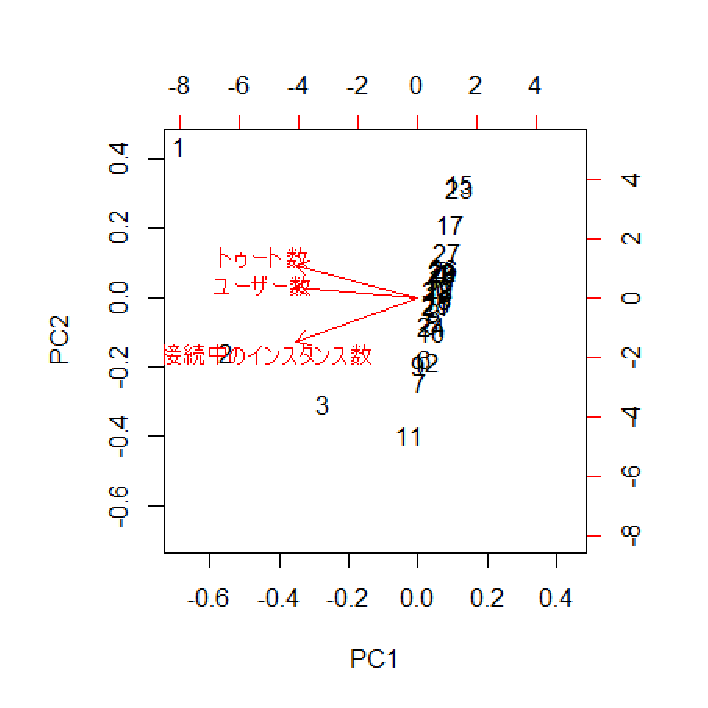
\includegraphics[width=7cm,clip]{R1.pdf}
\caption{ユーザー数,トゥート数,接続中のインスタンス数を主成分分析した結果}\label{R}
\end{figure}

\section{今後の計画}
今後の計画は以下のとおりに行う.
\begin{itemize}
\item データ数を増やし,再度主成分分析を行う.

\item TwitterとMastodonのつぶやきをベクトル化し,定量的に違いを調査する.
\end{itemize}

\bibliographystyle{junsrt}
\bibliography{biblio}%「biblio.bib」というファイルが必要.

\end{document}
